\section{A More Robust Approach to \glsentryshort{tpc} Readout Wires}
\label{sec:studies_cuoka}

As outlined in Section~\ref{sec:lartpc_challenges} classical wire readouts pose two big challenges to future \lartpc{}s: ambiguities and mechanical stability.
A possible solution to the mechanical problems with wires is to not use actual wires but instead print thin coper tracks on a support structure.
I investigated this solution and provide a proof of concept in this section.

In a classical wire readout plane the induction signal is produced by drifting the charge through one or multiple induction wire grids.
With the proposed scheme of copper tracks on a support structure it is no longer possible for the charge to actually drift through the induction plane(s).
Therefore, induction is only produced by the approach of the charge.
One consequence of this is that induction signals will no longer bi bipolar.
As opposed to the classic design the collection plane will even be in front of the induction plane(s).
This means that the charge can only approach the induction plane(s) until it is collected by the collection plane on the top layer of the support structure.
That is why it is crucial to make the support structure as thin as possible in order to get induction signals as high as possible.
Using a \gls{fr4} structure as in classical \gls{pcb} designs is not a viable option.
Very thin support structures can be provided by using a flexible \gls{pcb} made from Kapton instead of \gls{fr4}.
These can be made as thin as a few \SI{10}{\micro\metre}.
For this test a Kapton layer of \SI{50}{\micro\metre} was used with a single induction plane on the back (Fig.~\ref{fig:cuoka_readout-plane}).
The Kapton layer is supported by an \gls{fr4} frame for mounting on the \gls{tpc}.

\begin{figure}[htb]
	\centering
	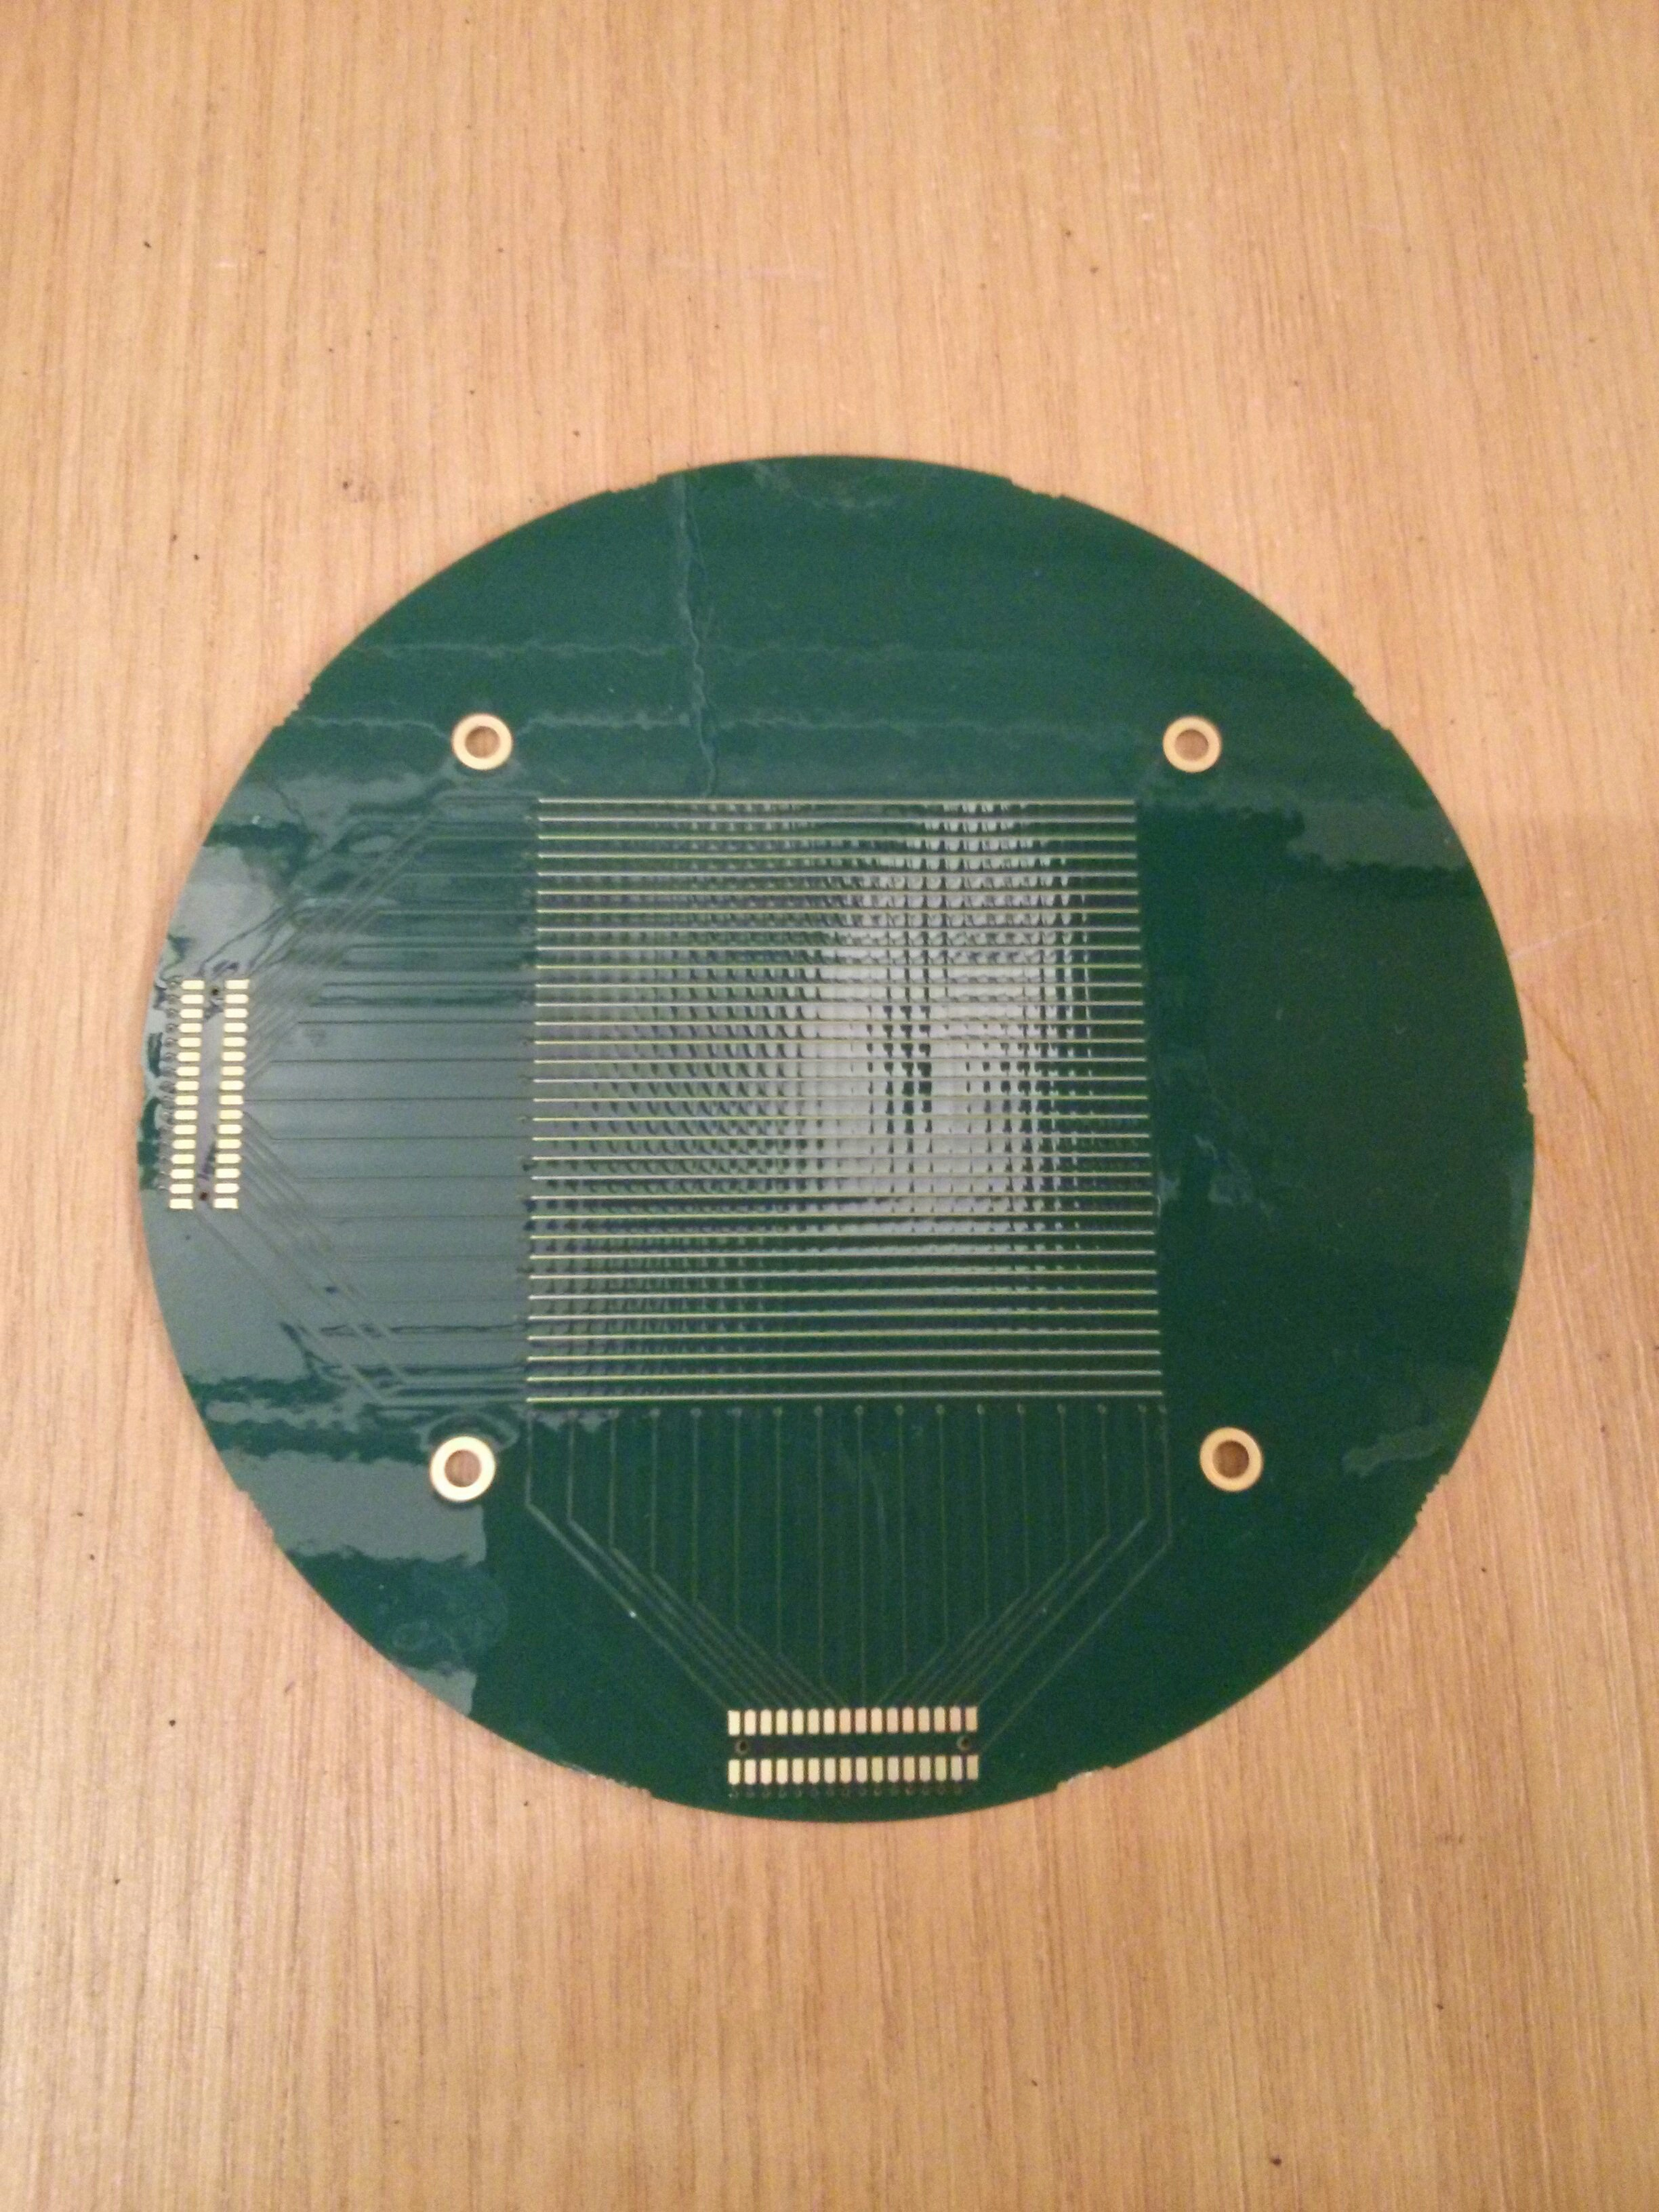
\includegraphics[width=0.5\textwidth]{cuoka/readout_plane_bottom}
	\caption[Copper on Kapton readout plane]{%
		Copper on Kapton readout plane.
	}
	\label{fig:cuoka_readout-plane}
\end{figure}

The test was performed in a small vacuum-insulated double-bath cryostat with an inner volume of \SI{15}{\centi\metre} diameter and \SI{60.8}{\centi\metre} height.
Prior to filling the cryostat was evacuated using a turbo-molecular pump and then purged with argon gas and evacuated a second time.
From earlier experiments~\cite{2photonAbs} the purity can be assumed to be $\sim{\SI{1}{ppb}}$ after filling.
The cryostat is sealed using rubber O-rings, which lose tightness at cryogenic temperatures.
Therefore, and due to the fact that no purification system was available, the purity degraded slowly in the course of the experiment.
The \SI{8}{\centi\metre} long field cage consists of \num{8} copper rings of \SI{8}{\centi\metre} diameter terminated by a copper plate cathode.
A field of \SI{1}{\kilo\volt\per\centi\metre} is generated using a resistive divider.

\begin{figure}[htb]
	\centering
	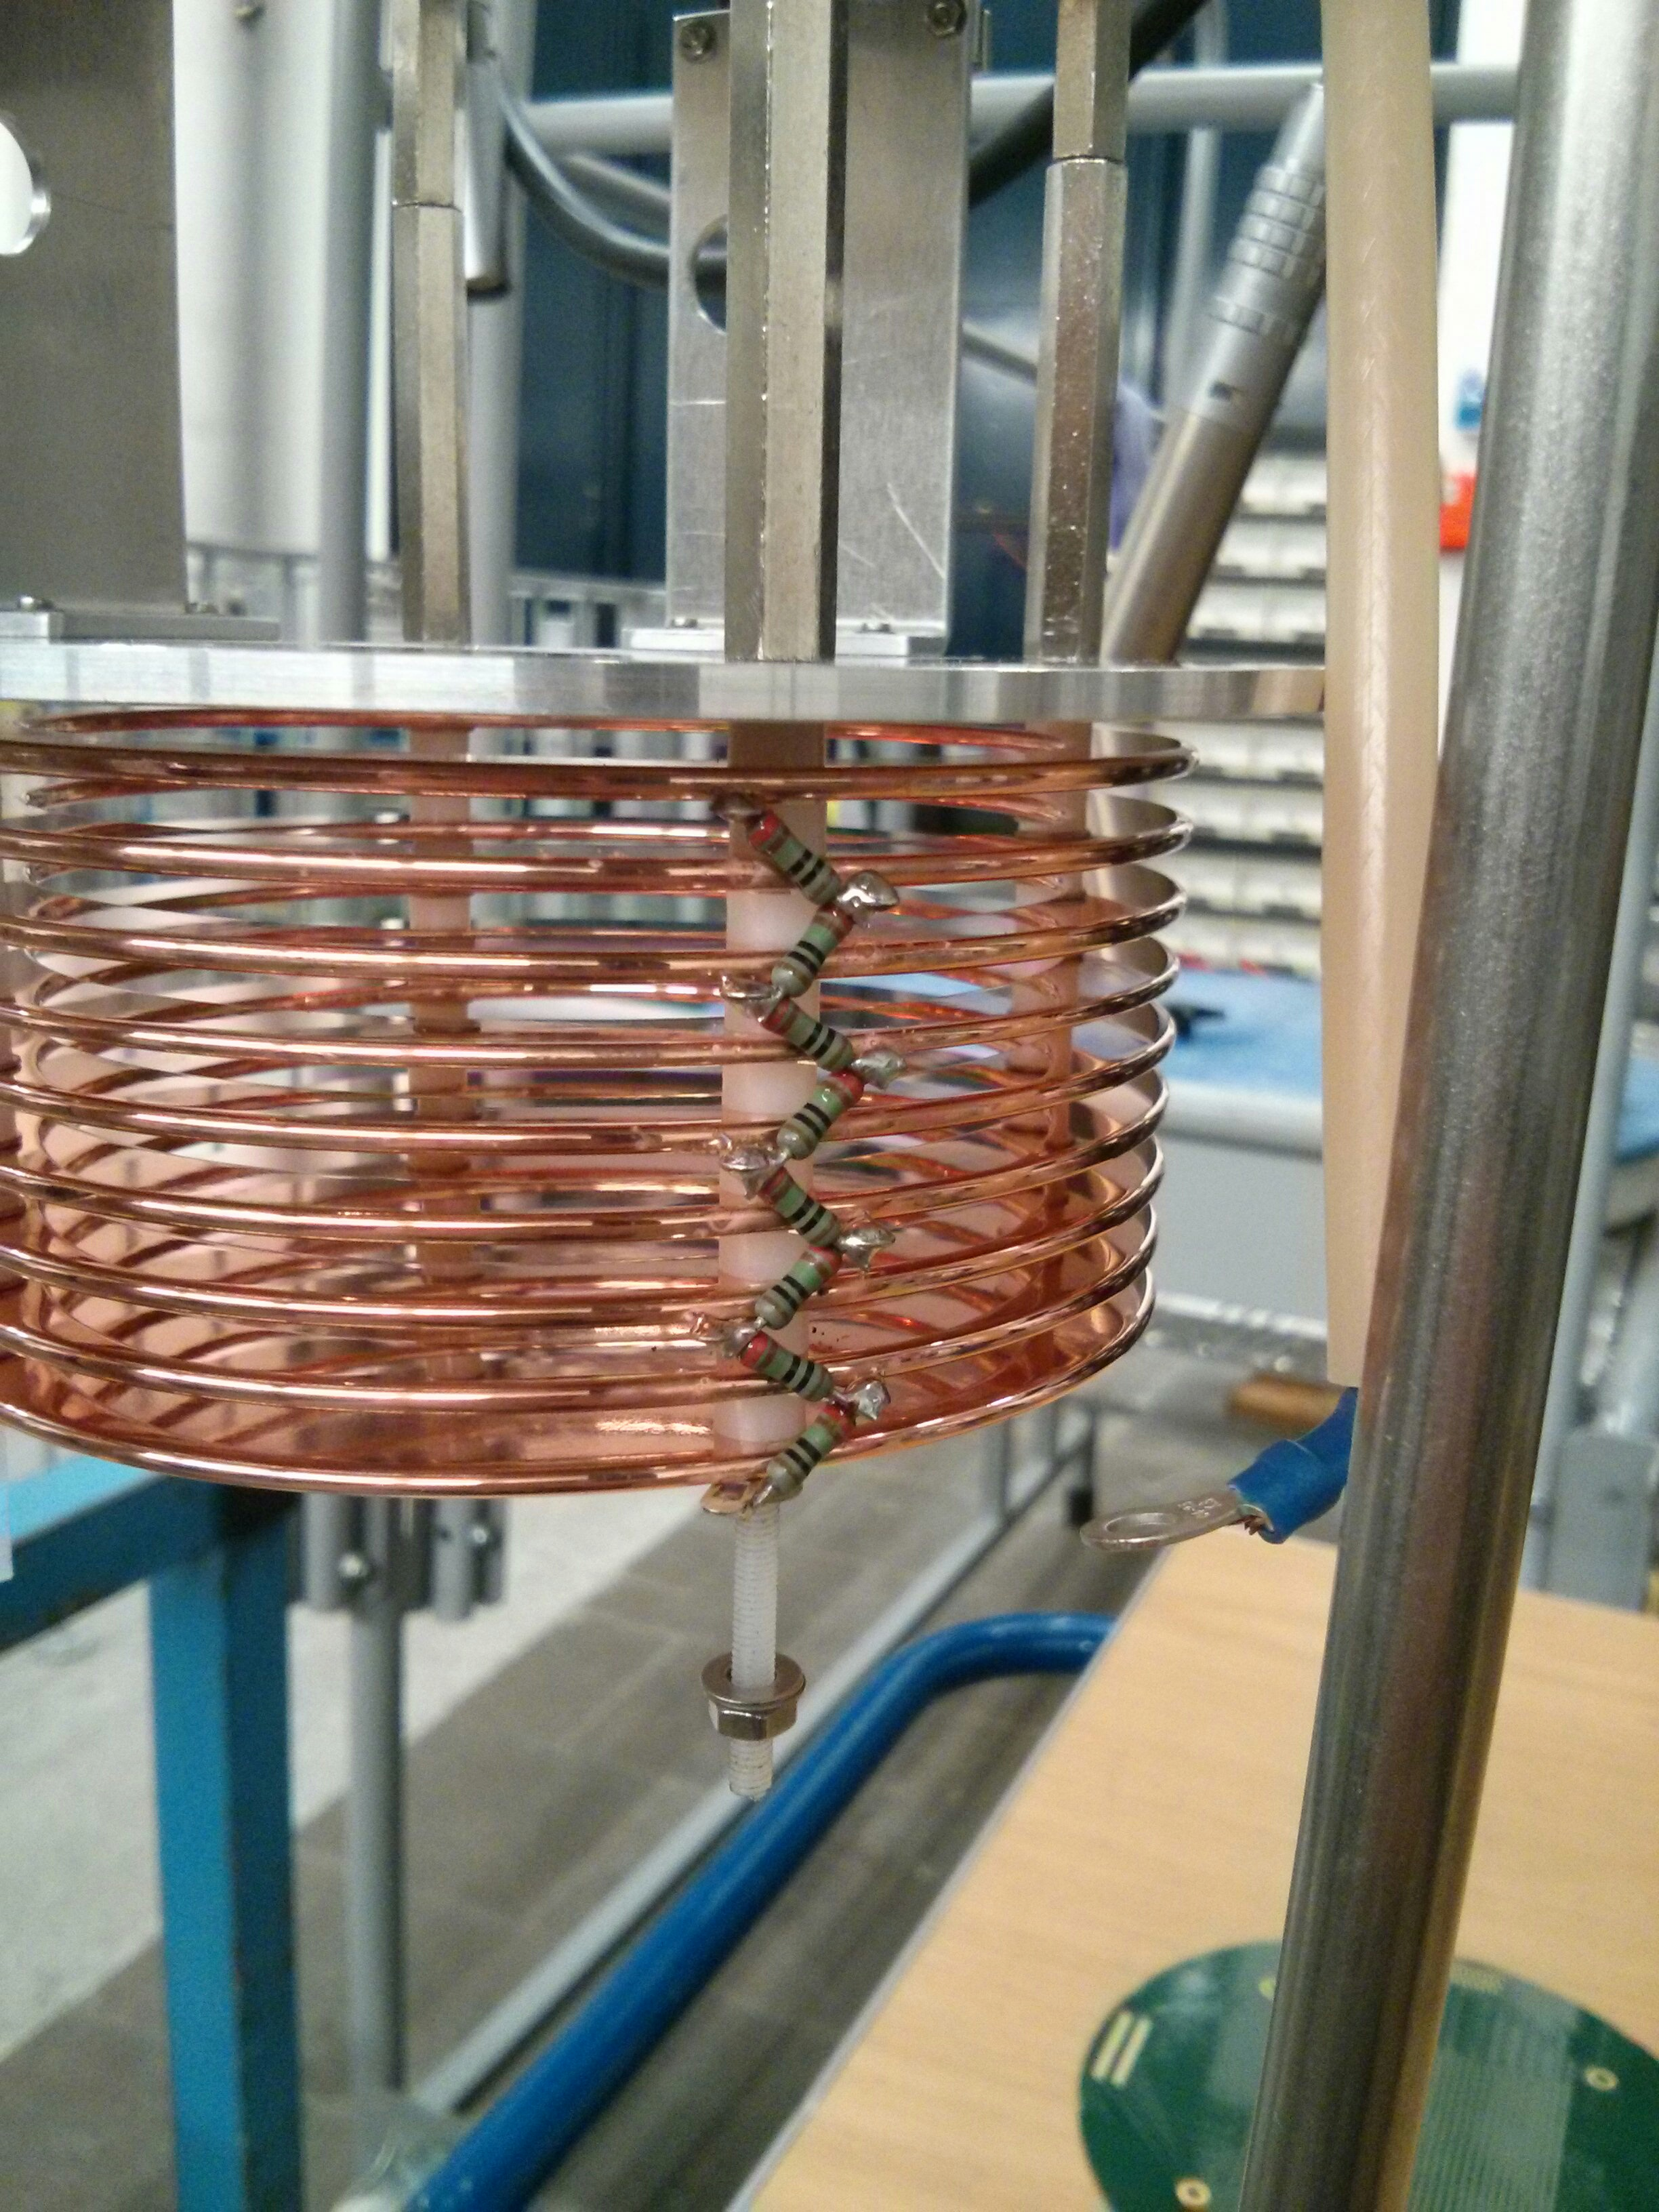
\includegraphics[width=0.5\textwidth]{cuoka/tpc}
	\caption[Copper on Kapton test \glsentryshort{tpc}]{%
		\acrshort{tpc} used for the copper on Kapton readout test.
	}
	\label{fig:cuoka_tpc}
\end{figure}

The charge readout electronics were adopted from \AT{} without modifications.
Charge signals are amplified by cryogenic charge amplifiers and then digitised at room temperature.
More details can be found in Section~\ref{sec:studies_at-ro}.

No internal light trigger system could be used due to the limited space inside the cryostat.
Instead, the digitisers were either triggered on one of the charge collection channels or by an external muon telescope.
The latter was formed of two scintillator panels with \glspl{pmt} above and below the cryostat, respectively.
Triggering directly on charge collection channels has the potential disadvantage of recording events only partially.
If the triggering channel does not receive the first charge pulse of the event, all earlier pulses are lost, unless the \gls{daq} implements a pre-trigger ring buffer of sufficient size.
It is therefore preferable to trigger on the external muon telescope.

Using the above-described setup cosmic muons were recorded over the course of multiple hours.
A typical event is depicted in Figure~\ref{fig:cuoka_event}.
It can be seen that due to the event being almost parallel to the induction strips the induction signal is in fact stronger than the collection signal.
The reason for the bad \gls{snr} is improper grounding of the setup and high noise levels in the lab from the nearby train station and air conditioning.
No further analysis was performed on this data due to time constraints and the upcoming test of a pixelated readout described in Chapter~\ref{chap:dune-nd}.
Anyhow, the fact that cosmic muons could be seen using this setup proves that there is no inherent problem with having the induction plane a few \SI{10}{\micro\metre} behind the collection plane.

\begin{figure}[htb]
	\centering
	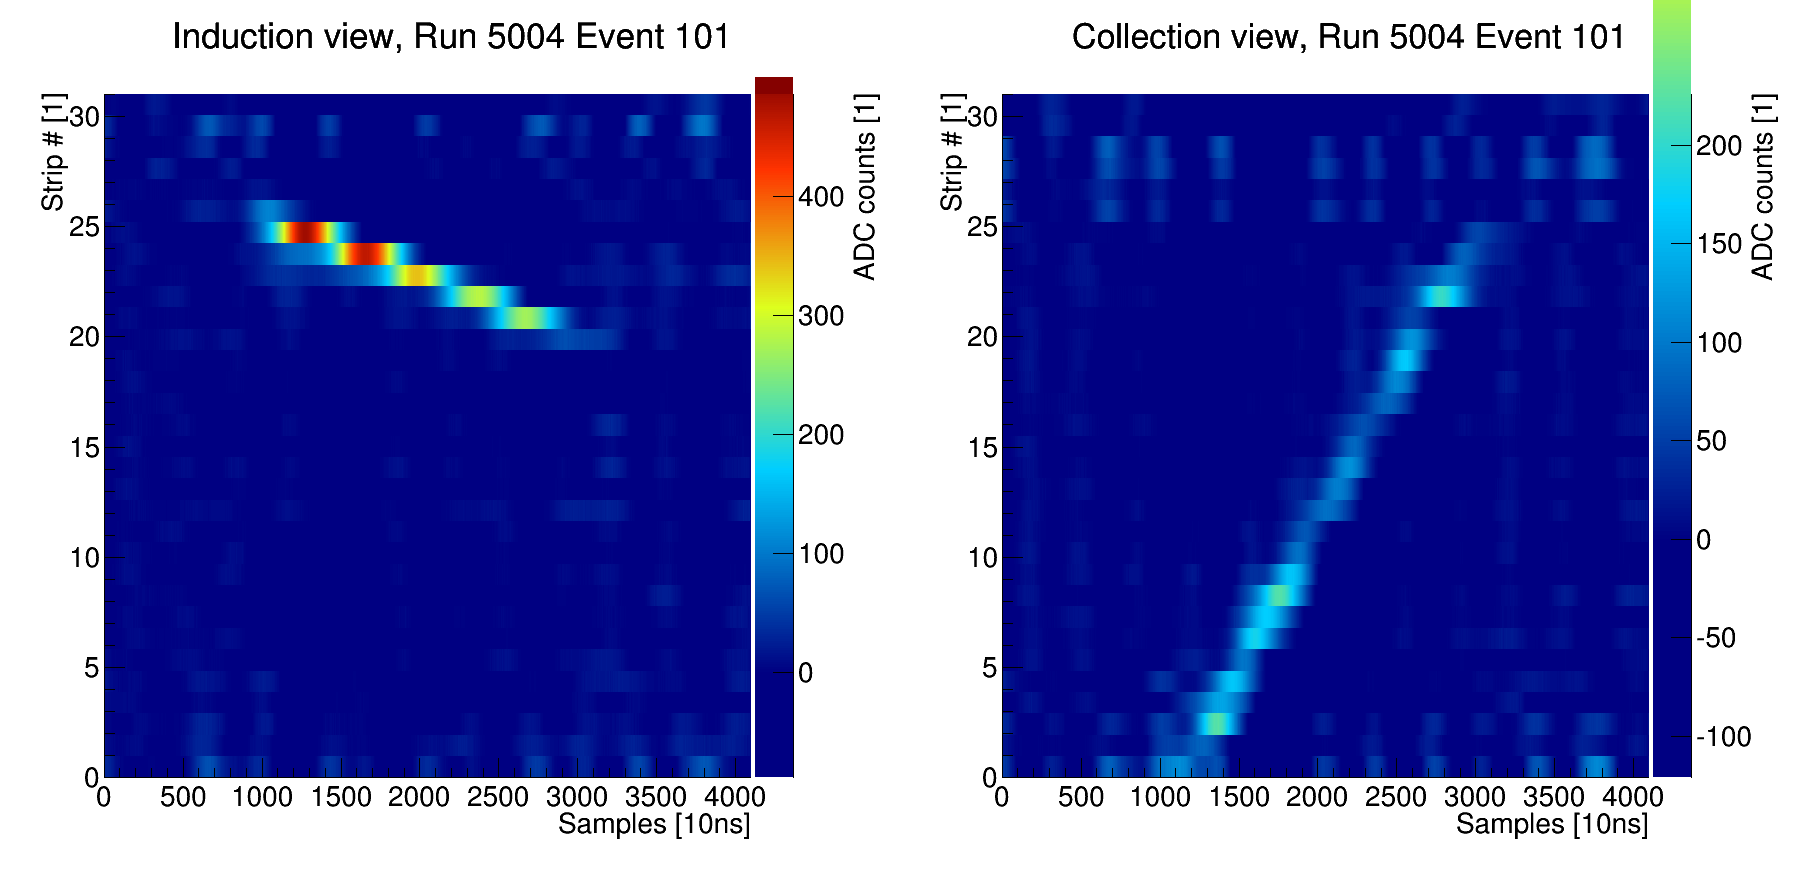
\includegraphics[width=\textwidth]{cuoka/muon_event}
	\caption[Copper on Kapton test muon event]{%
		Cosmic muon event recorded using the copper on Kapton readout.
	}
	\label{fig:cuoka_event}
\end{figure}

While this technique can potentially solve the mechanical problems of classical wire readouts, it does not reduce the ambiguities inherent to \gls{2d} projective readouts outlined in Section~\ref{sec:lartpc_challenges}.
Therefore, I decided not to further investigate copper on Kapton readouts, and instead focus on pixelated readouts for \lartpc{}s, providing real \gls{3d} data.


\section{Pixelated Charge Readouts}
\label{sec:studies_pixel-ro}

Wire readouts are not suitable for \lartpc{}s the size of the envisioned future neutrino detectors, as has been outlined in Section~\ref{sec:lartpc_challenges}.
The ambiguities caused by the nature of wire readouts can be eliminated by using a fully pixelated readout.
Such a readout will record a true \gls{2d} image of the charge for every time slice and thus directly produce \gls{3d} space points of the event.
On the other hand, this will increase the required number of \gls{daq} channels and therefore the data throughput.
To illustrate this let us imagine a readout plane of \SI{1 x 1}{\metre} and a desired resolution of \SI{5}{\milli\metre}.
For a conventional wire readout with two planes this results in

\begin{IEEEeqnarray}{rCl}
	\qty(\frac{\SI{1}{\metre}}{\SI{5}{\milli\metre}}) \times 2 & = & 40
\end{IEEEeqnarray}

wires and thus \gls{daq} channels.
In order to reduce ambiguities one can use more than two planes which will increase the number of channels linearly with the number of planes.
For a pixelated readout

\begin{IEEEeqnarray}{rCl}
	\qty(\frac{\SI{1}{\metre}}{\SI{5}{\milli\metre}}) ^ 2 & = & 400
\end{IEEEeqnarray}

\gls{daq} channels are required.
Scaling this up to the needed detector size leads to an enormous number of \gls{daq} channels and data throughput.

It is possible to reduce the number of channels by employing some form of multiplexing.
There are multiple options one could imagine for this:
\begin{itemize}
	\item Digital multiplexing
	\item Genetic multiplexing
	\item \glspl{roi}
\end{itemize}

Digital multiplexing means digitising all channels as close as possible to the readout plane and then mutliplexing the digital data onto a high-speed digital link.
An advantage of this technique is that the technology already exists and is well established in information technology.
Ideally, one would feed the data stream into an optical fibre, which additionally provides galvanic isolation of the readout from the \gls{daq}.
The challenging part is that all of this needs to happen at cryogenic temperatures, which is far from trivial because most off-the-shelf components are not made for this.
A detailed description of upcoming electronics capable of cold digitisation and multiplexing is given in Section~\ref{sec:studies_pixel-electronics}.
In contrast, genetic multiplexing and \glspl{roi} are forms of analogue multiplexing.
The difference to digital multiplexing is that multiple readout channels are combined into a single analogue link before digitising them at room temperature outside the cryostat.
In the two schemes described here this happens by connecting multiple readout channels to a single \gls{daq} channel.

In genetic multiplexing~\cite{gen_mux} the connections are done in a way that a certain event type (a single straight track for instance) forms a distinct pattern of \gls{daq} channels activated.
For simple events it is possible to recover the full event from the pattern.
Naturally, this reintroduces new ambiguities.
Depending on the complexity of the event topology and the degree of multiplexing they can potentially be resolved during reconstruction.
In any case, if the event is too complex, it cannot be reconstructed properly.
While genetic multiplexing has been shown to work for \gls{1d} readouts (wires), there is no known solution for two dimensions (pixels).

A third technique is to subdivide a pixelated readout plane into \glspl{roi}.
This scheme was tested for an earlier PhD thesis at \gls{help} using a \gls{micromegas} in a xenon gas \gls{tpc}~\cite{maplesyrup}.
All pixels at the same relative position inside the \glspl{roi} are connected to the same \gls{daq} channel.
For instance, let us assume squared \glspl{roi}.
One \gls{daq} channel would connect to all the pixels in the top left corners of the \glspl{roi}.
Another channel would connect to all the pixels in the top right corner and so on.
To explain this a little better let us assume a square pixel plane of $N \times N$ pixels, where $N = n ^ 2$ and $n$ integer.
Then, we divide the plane into $n \times n = N$ \glspl{roi}, each consisting of $n \times n = N$ pixels.
For such a readout we need $N$ \gls{daq} channels for the \glspl{roi} and another $N$ channels for the pixels.
We need only as many pixel channels as we have pixels per \gls{roi} because all the pixels at the same relative position inside the \glspl{roi} are connected together to one \gls{daq} channel.
This means that we can read out a $N \times N$ pixel plane using only $2 N$ \gls{daq} channels; the same number required by a conventional 2-plane wire readout of the same size and pitch.
If there is a signal on a certain \gls{daq} channel, the position inside the \gls{roi} is known but not the \gls{roi}.
To determine the full position each \gls{roi} has its own inductive grid in between the pixels.
The grid is biased such that the charge is fully focussed onto the pixels and does not collect any charge.
It is possible to disentangle the true position by combining the bipolar pulse on the \gls{roi} grid with the collection pulse from the pixels.
Again, the drawback of this approach is that it is not free of ambiguities.
It fails for multiple simultaneous hits when it is impossible to say which pixel pulse belongs to which \gls{roi} pulse.

Independently of the amount of data one needs to bring out of the detector a second problem is heat dissipation.
The more of the readout chain is sitting inside of the detector, the more serious this problem becomes.
It is especially problematic for digital multiplexing which requires a lot of cryogenic electronics.
A possible solution to this is to power only that part of the readout that is actually needed.
This would require a means to wake up the part of the readout where the charge is arriving before it is collected.
Provided the wake-up time is short enough, inductive grids on \glspl{roi} could allow precisely for this.


\section{Charge Readout Summary}
\label{sec:studies_charge-ro-summary}

Replacing a classical wire readout by copper strips on a thin ($\sim \SI{10}{\micro\metre}$) layer of Kapton can alleviate the mechanical challenges met by the charge readout.
However, this does not change the projective nature of the readout, introducing ambiguities in event reconstruction.
A pixelated readout can provide true \gls{3d} information at the price of an increased number of channels.
Due to the lack of bespoke pixel electronics able to readout so many channels (see Section~\ref{sec:studies_pixel-electronics}) I implemented a form of analogue multiplexing.
As the \gls{roi} approach had already been demonstrated in a gas \gls{tpc}, it was chosen for the first prototype of a pixelated \lartpc{}.
The readout plane can be realised as a conventional \gls{pcb} because the detector is a single-phase \lartpc{}, and thus no gas amplification as in \gls{micromegas} is needed.
Alongside the \gls{pcb} I designed a new \gls{tpc} which can be reused for future prototyping efforts.
The design of \gls{pcb} and \gls{tpc} as well as the results from the first tests will be described in Section~\ref{sec:ac_viper}.